\section{Smart Contract Runtime and Execution} \label{sec:Runtime}


\textit{This part has been updated to be Chang compatible. The code here is already compatible with DReps, the new Aiken version, and Plutus v3.}

\subsection{Overview of Cardano's Smart Contract Execution Model}

Smart contracts on Cardano are simple constructs based on \textbf{validator scripts}. These scripts define the logic or rules to be enforced by Cardano nodes when a transaction attempts to move a UTXO locked inside the script's address.

Validator scripts can access the \textbf{transaction context} (e.g., who signed it, and which assets are sent to/from where) and the \textbf{datum} of the locked UTXO being moved, allowing the creation of complex contracts. For instance:
\begin{quote}
With smart contracts, we can add conditions to stake delegation, withdraw Cardano rewards from the protocol, or create minting policies with more dynamic conditions than regular ones.
\end{quote}

Validator scripts are executed with three main arguments:
\begin{itemize}
    \item \textbf{Datum:} Attached to the output locked by the script, often carrying state.
    \item \textbf{Redeemer:} Attached to the spending input, typically providing an input to the script. For example, a validator can apply the redeemer to the datum and verify it matches the output UTXO datum.
    \item \textbf{Context:} Contains transaction-level information, used to assert properties like “Bob signed it.”
\end{itemize}

\textbf{Transaction context properties:}
\begin{center}
\begin{tabular}{|l|p{10cm}|}
\hline
\textbf{Property} & \textbf{Description} \\
\hline
\textbf{inputs} & Outputs to be spent. \\
\textbf{reference inputs} & Inputs used for reference only, not spent. \\
\textbf{outputs} & New outputs created by the transaction. \\
\textbf{fees} & Transaction fees. \\
\textbf{minted value} & Minted or burned value. \\
\textbf{certificates} & Digest of certificates in the transaction. \\
\textbf{withdrawals} & Used to withdraw rewards from the stake pool. \\
\textbf{valid range} & Time range in which the transaction is valid. \\
\textbf{signatories} & List of transaction signatures. \\
\textbf{redeemers} & Data used as input to the script. \\
\textbf{id} & Transaction identification. \\
\hline
\end{tabular}
\end{center}

\subsection{Understanding the Transaction Context Table}

\textbf{Inputs:} These represent UTXOs being \textit{spent} in the transaction. In the UTXO model, every transaction produces outputs, which in turn become inputs for future transactions. Understanding this flow is key to interpreting inputs and outputs.

\textbf{Outputs:} These are the new UTXOs created by the transaction, ready to be used as inputs in subsequent transactions.

\textbf{Fees:} The amount of lovelace spent for transaction execution. This value is predictable and depends on the transaction size. Fees can often be optimized.

\textbf{Minted Value:} This indicates any minting or burning of tokens that occurs in the transaction.

\textbf{Certificates:} Information about stake operations. For example:
\begin{itemize}
    \item Registering a stake key.
    \item Delegating to a DRep.
\end{itemize}

\textbf{Withdrawals:} Rewards withdrawn from stake keys. For example, if you use a wallet like Lace, which allows delegation to multiple pools, you may see multiple withdrawals in one transaction.

\textbf{Valid Range:} A time frame during which the transaction is valid. This is useful for ensuring a transaction only executes within specific boundaries.

\textbf{Signatories:} A list of hashes representing who signed the transaction. This is essential for multi-signature transactions.

\textbf{Redeemers:} A list of redeemers used by the contracts executed in the transaction.

\textbf{ID:} The transaction hash, uniquely identifying the transaction.

During runtime, each validator checks its \textit{datum}, \textit{redeemer}, and the \textit{context} (or local transaction state).

\textbf{Important exercise:} 
Imagine a transaction that:
\begin{itemize}
    \item Spends \textbf{three different UTXOs} from the same contract.
    \item Withdraws staking rewards from a stake key contract.
    \item Mints \textbf{two different tokens} under separate contract policies.
\end{itemize}

\textit{Questions:}
\begin{enumerate}
    \item How many unique contracts are executed?
    \item How many datums are present?
    \item How many redeemers?
\end{enumerate}

\textbf{Answer:} After a blank page—\textit{Take your time; don’t rush!}
\newpage
\thispagestyle{empty}
\textbf{Real answer:}

\begin{enumerate}
    \item 4
    \item 3
    \item 6
\end{enumerate}

Did you get them? Let's try to understand why.
Spending inputs from a contract, even if it's coming from the same contract is treated like a unique execution.
Therefore for each input coming from contract A, we will have it's own Datum and it's own redeemer. 

Withdraw and minting contract do not have datums, they have redeemers.
You can mint or withdraw from the same contract only once, therefore the logic behind these contracts must be more flexible to allow different logic inside the same execution.

It will be easier to understand at the end of this chapter, you need to take home this:

\begin{quote}
    SPEND contracts are executed once for each input, while minting and withdrawals contracts are executed once for each transaction
\end{quote}



\section{Transaction Verification and Script Validation}


To understand transaction validation on Cardano, it is crucial to recognize that even if a script validates a transaction, the transaction might still fail due to the network's robust two-phase validation mechanism. This section explores this process and the role of collateral in ensuring successful smart contract execution.

\subsubsection{Two-Phase Validation Mechanism}

Cardano employs a two-phase validation scheme to minimize uncompensated work for nodes, ensuring efficiency and security:

\begin{itemize}
    \item \textbf{Phase 1: Structural Validation}
    \begin{itemize}
        \item Checks if the transaction is correctly constructed.
        \item Ensures that the transaction can pay its processing fee.
        \item If Phase 1 fails, the transaction is immediately discarded without running any scripts.
    \end{itemize}
    \item \textbf{Phase 2: Script Execution}
    \begin{itemize}
        \item Executes the scripts included in the transaction.
        \item If a script fails, the transaction fails, and collateral is used to compensate nodes.
    \end{itemize}
\end{itemize}

\subsubsection{The Role of Collateral}
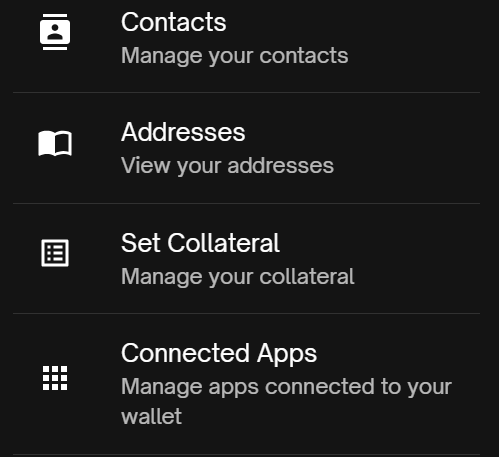
\includegraphics{collateral.png}

Collateral ensures that nodes are compensated for their work if Phase 2 validation fails. It acts as a monetary guarantee, encouraging careful design and testing of smart contracts. Key details about collateral:

\begin{itemize}
    \item \textbf{Collateral Inputs:} The collateral amount is determined by the total balance of UTXOs marked as collateral inputs.
    \item \textbf{Safety for Honest Users:} Collateral is not collected if a transaction succeeds or is invalid at Phase 1.
    \item \textbf{Deterministic Costs:} Cardano's deterministic design allows users to calculate execution costs and collateral requirements in advance, unlike Ethereum where gas costs can vary based on network activity.
    \item \textbf{Vasil Upgrade Improvement:} Developers can specify a change address for script collateral, ensuring only the required amount is taken if a script fails, with the remainder returned to the specified address.
\end{itemize}

\subsubsection{Importance of Collateral}

Without collateral, malicious actors could exploit the network by flooding it with invalid transactions at little cost. By requiring collateral, Cardano ensures:

\begin{itemize}
    \item Transactions calling non-native (Phase 2) smart contracts include sufficient collateral to cover potential failure costs.
    \item Denial of Service (DoS) attacks become prohibitively expensive.
    \item Honest users never lose their collateral as long as transactions are valid and successful.
\end{itemize}

\subsubsection{Technical Details}

Phase 2 scripts on Cardano can perform arbitrary computations and require a budget of execution units (ExUnits) to quantify resource usage. This budget is included in the transaction fee calculation. Collateral provides additional safeguards:

\begin{itemize}
    \item \textbf{Multi-Signature Scripts:} Introduced in the Shelley era, Phase 1 scripts follow deterministic ledger rules, enabling straightforward cost assessment.
    \item \textbf{ExUnit Budgeting:} Phase 2 scripts require a resource budget for metrics like memory usage and execution steps, ensuring fair cost allocation.
\end{itemize}

The Cardano testnet provides a safe environment with free test ADA, enabling developers to rigorously test smart contracts before deploying them on the mainnet. This ensures that transactions and scripts function correctly under real-world conditions.


\section{Debugging and Troubleshooting Smart Contracts}

Debugging smart contracts can be challenging, but interacting directly with the blockchain is not always necessary. Thanks to tools like Aiken and Gastronomy, developers can efficiently test and debug their smart contracts in a controlled environment.

\subsubsection{Debugging with Aiken}

Aiken offers first-class support for unit tests and property-based tests, allowing developers to write and execute tests directly in Aiken without deploying to the blockchain. The toolkit (`aiken check`) parses tests, runs them, and displays detailed reports.

\paragraph{Unit Tests}

Unit tests in Aiken are written using the `test` keyword. A test is a named function that takes no arguments and returns a boolean. It is valid (i.e., it passes) if it returns `True`.

\begin{verbatim}
test foo() {
  1 + 1 == 2
}
\end{verbatim}

Unit tests can call functions and use constants, and they execute on the same virtual machine used for on-chain contracts. This ensures that tests mirror the production environment.

\paragraph{Example Unit Tests}

\begin{verbatim}
lib/example.ak
fn add_one(n: Int) -> Int {
  n + 1
}
 
test add_one_1() {
  add_one(0) == 1
}
 
test add_one_2() {
  add_one(-42) == -41
}
\end{verbatim}

Running `aiken check` generates a report grouping tests by module and displaying the memory and CPU execution units needed for each test. This report can also be used as a benchmark to compare execution costs of different approaches.

Tests in Aiken can be as complex as necessary, without the execution limits imposed on on-chain scripts.

\paragraph{Trace and Debugging}

Aiken supports debugging via CBOR diagnostic traces. Developers can use `trace` to print diagnostic data (e.g., integers or byte arrays) in the event of a contract failure. If the contract succeeds, no output is shown.

\begin{verbatim}
// An Int becomes a CBOR int
trace cbor.diagnostic(42)
 
// A ByteArray becomes a CBOR bytestring
trace cbor.diagnostic("foo")
\end{verbatim}

This feature provides valuable insights during debugging by simulating breakpoints.

\subsubsection{Advanced Debugging with Gastronomy}

\includegraphics[scale=0.3]{gastronomy.png}
Gastronomy, developed by Sundae Labs, is a powerful UPLC debugger designed to aid in diagnosing failed scripts based on error codes. It allows developers to step through script execution with ease.

\paragraph{Features}

\begin{itemize}
    \item Stores the state of the machine at every execution step.
    \item Allows stepping forward and backward to analyze script behavior.
    \item Provides a user-friendly interface for debugging.
\end{itemize}

\paragraph{Quick Start}

\textbf{CLI Tool:}
\begin{verbatim}
gastronomy-cli run test_data/fibonacci.uplc 03
N - Advance to the next step
P - Rewind to the previous step
Q - Quit
\end{verbatim}

\textbf{GUI Tool:}
Simply run `gastronomy` to launch the graphical interface.

\paragraph{Configuration}

Gastronomy can be configured using environment variables or a `.gastronomyrc.toml` file in the home directory. Example configuration:

\begin{verbatim}
    Setting          Environment Variable     Description
    blockfrost.key   BLOCKFROST_KEY           The API key to use when querying Blockfrost.
\end{verbatim}




By leveraging Aiken and Gastronomy, developers can thoroughly test and debug their smart contracts, ensuring reliability and efficiency before deployment.


\section{Tx Optimization Techniques for Efficient Execution}

In recent years, several effective techniques have been discovered to optimize smart contracts on Cardano. Many of these can be found in the repository at \href{https://github.com/Anastasia-Labs/aiken-design-patterns}{Aiken Design Patterns}. Here, we will discuss two game-changing techniques: the "Withdraw 0 Trick" and "Parametric Scripts."

\subsubsection{Withdraw 0 Trick}

The "Withdraw 0 Trick" is particularly useful for validators that need to handle multiple inputs efficiently. By splitting logic into two distinct parts—a minimal spending logic and an arbitrary withdrawal logic—scripts can be made significantly more efficient. 

\paragraph{How It Works}

Withdraw scripts are executed only once per transaction, whereas spend validators are executed once for every input originating from the same smart contract. For example, if purchasing multiple NFTs from a marketplace, the transaction's execution logic grows proportionally to the number of NFTs.

Using the "Withdraw 0 Trick," this logic is split:
\begin{itemize}
    \item The spend validator checks that a "withdraw 0" operation is executed.
    \item The withdrawal logic is handled independently in the "withdraw 0" contract, decoupling it from the number of NFTs.
\end{itemize}

This approach reduces complexity, ensures scalability, and maintains elegance in design.

\paragraph{Implementation Details}

The module offers two key functions for spending endpoints:
\begin{itemize}
    \item \textbf{spend} \textendash{} Traverses both the withdrawals and redeemers fields, validating against both the redeemer and the withdrawal quantity.
    \item \textbf{spend\_minimal} \textendash{} Traverses only the withdrawals, ideal when no validation is needed on the staking script's redeemer or withdrawal quantity.
\end{itemize}

Additionally, the \textbf{withdraw} function unwraps the staking credential and provides the underlying hash, facilitating minimal execution logic.

\subsubsection{Parametric Scripts}

Parametric scripts are another crucial optimization technique, significantly enhancing execution efficiency by predefining key parameters within the script itself.

\paragraph{Why Use Parametric Scripts?}

Certain contracts require specific parameters, such as a spend contract that must identify an NFT with a matching policy script hash. Without predefined parameters, the contract would consume excessive CPU resources to compute its own script hash. By using parametric scripts, the contract already "knows" the required values, saving computation time and resources.

\paragraph{Practical Example}

Consider a minting script that restricts token destinations to instances of a specific spending script parameterized by user wallets. Each wallet results in a different script address, making verification challenging. Using parametric scripts, the minting script can:
\begin{itemize}
    \item Validate instances as the result of applying specific parameters to a parameterized script.
    \item Ensure robust asset flow control.
\end{itemize}

\paragraph{On-Chain Validation Requirements}

To validate parameterized scripts on-chain, the following restrictions apply:
\begin{itemize}
    \item Script parameters must have constant lengths (achieved via hashing).
    \item Redeemers must supply resolved values of parameters for each transaction.
    \item Dependent scripts must include CBOR bytes of instances before and after parameter application.
    \item Logic wrapping ensures a single occurrence of each parameter.
\end{itemize}

\paragraph{Implementation Steps}

Define parameterized scripts and generate instances with dummy data to obtain required prefix and postfix values. Use these values in your target script. For detailed examples, refer to \href{https://github.com/Anastasia-Labs/aiken-design-patterns}{validators/apply-params-example.ak}.

These optimization techniques provide a solid foundation for efficient, scalable smart contract execution on Cardano.
